% This file was created by matplotlib2tikz v0.6.18.
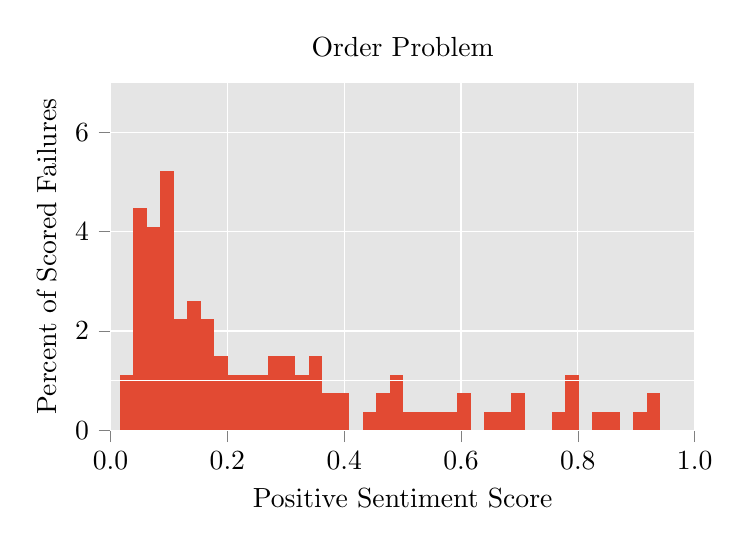
\begin{tikzpicture}

\definecolor{color0}{rgb}{0.886274509803922,0.290196078431373,0.2}

\begin{axis}[
axis background/.style={fill=white!89.80392156862746!black},
axis line style={white},
height=6cm,
tick align=outside,
tick pos=left,
title={Order Problem},
width=9cm,
x grid style={white},
xlabel={Positive Sentiment Score},
xmajorgrids,
xmin=0, xmax=1,
xtick={0,0.2,0.4,0.6,0.8,1},
xticklabels={0.0,0.2,0.4,0.6,0.8,1.0},
y grid style={white},
ylabel={Percent of Scored Failures},
ymajorgrids,
ymin=0, ymax=7
]
\draw[fill=color0,draw opacity=0] (axis cs:0.0153715908527374,0) rectangle (axis cs:0.0385056175291538,1.11792336575292);
\draw[fill=color0,draw opacity=0] (axis cs:0.0385056212544441,0) rectangle (axis cs:0.0616396479308605,4.47169346301168);
\draw[fill=color0,draw opacity=0] (axis cs:0.0616396479308605,0) rectangle (axis cs:0.0847736746072769,4.09905168102056);
\draw[fill=color0,draw opacity=0] (axis cs:0.0847736746072769,0) rectangle (axis cs:0.107907697558403,5.21697654694074);
\draw[fill=color0,draw opacity=0] (axis cs:0.107907697558403,0) rectangle (axis cs:0.131041720509529,2.23584709154603);
\draw[fill=color0,draw opacity=0] (axis cs:0.131041705608368,0) rectangle (axis cs:0.154175743460655,2.60848659328361);
\draw[fill=color0,draw opacity=0] (axis cs:0.154175758361816,0) rectangle (axis cs:0.177309781312943,2.23584709154603);
\draw[fill=color0,draw opacity=0] (axis cs:0.177309781312943,0) rectangle (axis cs:0.200443804264069,1.49056472769736);
\draw[fill=color0,draw opacity=0] (axis cs:0.200443804264069,0) rectangle (axis cs:0.223577827215195,1.11792354577302);
\draw[fill=color0,draw opacity=0] (axis cs:0.223577827215195,0) rectangle (axis cs:0.246711850166321,1.11792354577302);
\draw[fill=color0,draw opacity=0] (axis cs:0.24671183526516,0) rectangle (axis cs:0.269845843315125,1.11792354577302);
\draw[fill=color0,draw opacity=0] (axis cs:0.269845902919769,0) rectangle (axis cs:0.292979925870895,1.49056472769736);
\draw[fill=color0,draw opacity=0] (axis cs:0.292979896068573,0) rectangle (axis cs:0.316113948822021,1.49056280748515);
\draw[fill=color0,draw opacity=0] (axis cs:0.316113948822021,0) rectangle (axis cs:0.339247971773148,1.11792354577302);
\draw[fill=color0,draw opacity=0] (axis cs:0.33924800157547,0) rectangle (axis cs:0.362382024526596,1.49056472769736);
\draw[fill=color0,draw opacity=0] (axis cs:0.362381994724274,0) rectangle (axis cs:0.3855160176754,0.745282363848678);
\draw[fill=color0,draw opacity=0] (axis cs:0.385516047477722,0) rectangle (axis cs:0.408650070428848,0.745282363848678);
\draw[fill=color0,draw opacity=0] (axis cs:0.408650040626526,0) rectangle (axis cs:0.431784063577652,0);
\draw[fill=color0,draw opacity=0] (axis cs:0.431784093379974,0) rectangle (axis cs:0.4549181163311,0.372641181924339);
\draw[fill=color0,draw opacity=0] (axis cs:0.454918086528778,0) rectangle (axis cs:0.478052139282227,0.745281403742573);
\draw[fill=color0,draw opacity=0] (axis cs:0.478052139282227,0) rectangle (axis cs:0.50118613243103,1.11792498593588);
\draw[fill=color0,draw opacity=0] (axis cs:0.50118613243103,0) rectangle (axis cs:0.524320185184479,0.372640701871287);
\draw[fill=color0,draw opacity=0] (axis cs:0.524320185184479,0) rectangle (axis cs:0.547454178333282,0.372641661978628);
\draw[fill=color0,draw opacity=0] (axis cs:0.547454237937927,0) rectangle (axis cs:0.570588290691376,0.372640701871287);
\draw[fill=color0,draw opacity=0] (axis cs:0.570588231086731,0) rectangle (axis cs:0.593722283840179,0.372640701871287);
\draw[fill=color0,draw opacity=0] (axis cs:0.593722283840179,0) rectangle (axis cs:0.616856276988983,0.745283323957256);
\draw[fill=color0,draw opacity=0] (axis cs:0.616856336593628,0) rectangle (axis cs:0.639990389347076,0);
\draw[fill=color0,draw opacity=0] (axis cs:0.639990329742432,0) rectangle (axis cs:0.663124322891235,0.372641661978628);
\draw[fill=color0,draw opacity=0] (axis cs:0.663124322891235,0) rectangle (axis cs:0.686258375644684,0.372640701871287);
\draw[fill=color0,draw opacity=0] (axis cs:0.686258375644684,0) rectangle (axis cs:0.709392368793488,0.745283323957256);
\draw[fill=color0,draw opacity=0] (axis cs:0.709392428398132,0) rectangle (axis cs:0.732526481151581,0);
\draw[fill=color0,draw opacity=0] (axis cs:0.732526421546936,0) rectangle (axis cs:0.75566041469574,0);
\draw[fill=color0,draw opacity=0] (axis cs:0.75566041469574,0) rectangle (axis cs:0.778794467449188,0.372640701871287);
\draw[fill=color0,draw opacity=0] (axis cs:0.778794527053833,0) rectangle (axis cs:0.801928579807281,1.11792210561386);
\draw[fill=color0,draw opacity=0] (axis cs:0.801928520202637,0) rectangle (axis cs:0.82506251335144,0);
\draw[fill=color0,draw opacity=0] (axis cs:0.82506251335144,0) rectangle (axis cs:0.848196566104889,0.372640701871287);
\draw[fill=color0,draw opacity=0] (axis cs:0.848196566104889,0) rectangle (axis cs:0.871330559253693,0.372641661978628);
\draw[fill=color0,draw opacity=0] (axis cs:0.871330618858337,0) rectangle (axis cs:0.894464671611786,0);
\draw[fill=color0,draw opacity=0] (axis cs:0.894464612007141,0) rectangle (axis cs:0.917598605155945,0.372641661978628);
\draw[fill=color0,draw opacity=0] (axis cs:0.917598605155945,0) rectangle (axis cs:0.940732657909393,0.745281403742573);
\path [draw=white, fill opacity=0] (axis cs:0,0)
--(axis cs:0,7);

\path [draw=white, fill opacity=0] (axis cs:1,0)
--(axis cs:1,7);

\path [draw=white, fill opacity=0] (axis cs:0,0)
--(axis cs:1,0);

\path [draw=white, fill opacity=0] (axis cs:0,1)
--(axis cs:1,1);

\end{axis}

\end{tikzpicture}